\section{Results}
\label{sec:results}

The recovery head reaches $r = 8.34$ on the smaller 2x2 configuration
and $r = 6.96$ on the larger 2x4 configuration. Both numbers are well
above $1$, the threshold above which the head's predictions improve
on the all-zero baseline.

\begin{figure}[t]
  \centering
  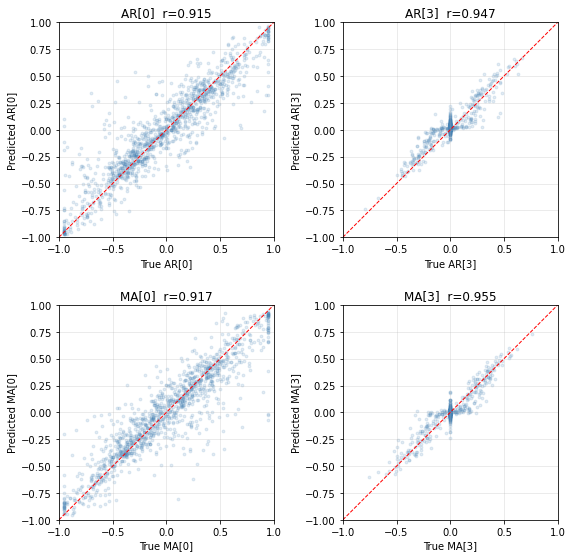
\includegraphics[width=0.78\linewidth]{figures/recovery_scatter_main.png}
  \caption{Recovery quality on the 2x4 (ARMA(4, 4)) configuration:
    predicted vs ground-truth coefficient for the four extreme
    positions AR$_0$, AR$_3$, MA$_0$, MA$_3$. Each subplot is a scatter
    of $300$ test samples, with the identity reference line and the
    Pearson correlation $r$ between predicted and true coefficients.}
  \label{fig:recovery-main}
\end{figure}

Figure~\ref{fig:recovery-main} shows the predicted vs ground-truth
coefficient on the 2x4 setup for the four extreme positions: AR$_0$,
AR$_3$, MA$_0$, MA$_3$. The Pearson correlation $r$ between predicted
and true coefficients sits between $0.91$ and $0.96$ on these four
positions.

The full 8-coefficient scatter for 2x4, the equivalent for 2x2, the
per-sample error distributions, and the per-coefficient table are
reported in Appendix~\ref{sec:appendix-graphs}.

\paragraph{Random-walk correlations.}
On the experiment of Section~\ref{sec:exp-corr}, the recovery head achieves
a mean Pearson $r = 0.962$ across all six pairwise correlations on an
800-sample test set ($52.4\times$ the MSE of the all-zero baseline;
$13.0\times$ the MSE of the mean-prediction baseline).

\begin{figure}[t]
  \centering
  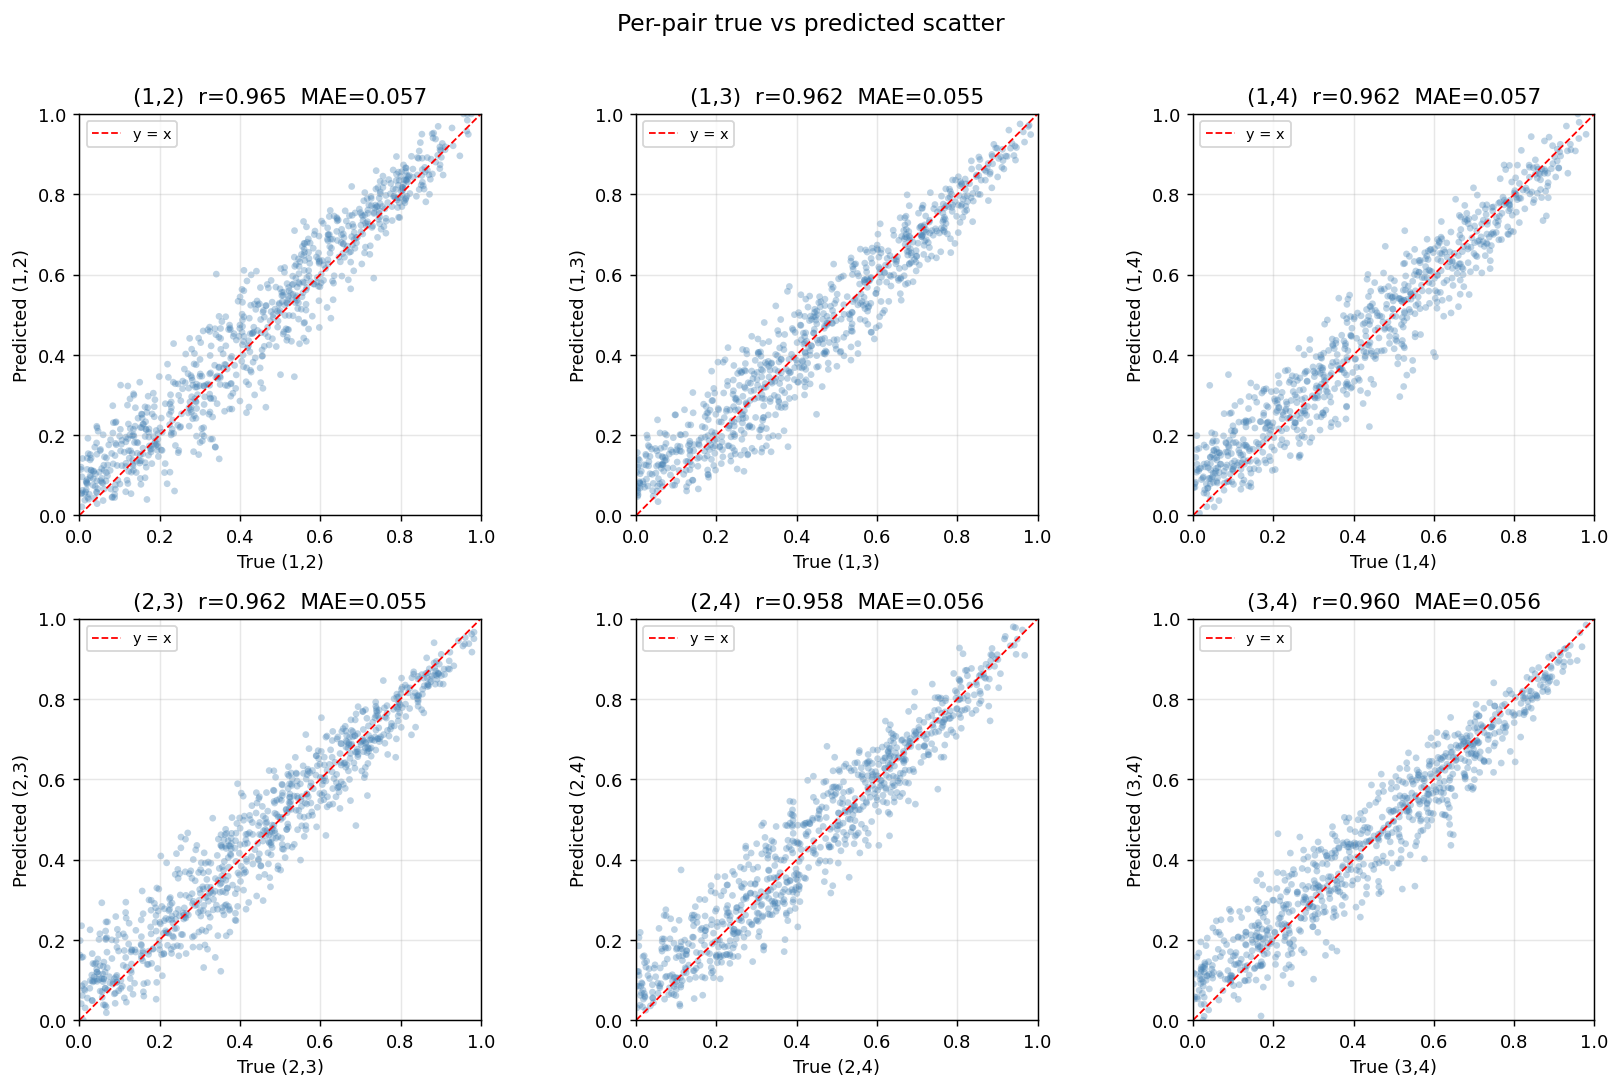
\includegraphics[width=\linewidth]{figures/corr_scatter_per_pair.png}
  \caption{Per-pair recovery for the random-walk correlation experiment:
    predicted vs.\ true correlation for each of the six off-diagonal
    entries of $\Sigma$.  Each subplot is a scatter of $800$ test
    samples with the identity reference line and Pearson $r$.  All six
    pairs lie in $r \in [0.958, 0.964]$.}
  \label{fig:corr-scatter}
\end{figure}

Figure~\ref{fig:corr-scatter} shows the per-pair scatter; the uniform
sampler produces even coverage across $[0, 1]$.  Full diagnostics and a
comparison against analytic baselines are in
Appendix~\ref{sec:appendix-corr}.
